\documentclass[a4paper]{article}
\usepackage[english]{babel}
\usepackage[top=1.1cm,headsep=0cm,bottom=1.1cm,footskip=0cm,left=1cm,right=1cm]{geometry}
\usepackage{multicolrule} %다단 본문
\usepackage{fontspec}
\setmathtt{exprdgs-italic.ttf}[BoldFont = exprdgs-bolditalic.ttf]
\usepackage[colorlinks=true, allcolors=black]{hyperref}
\usepackage{wrapfig} %문단 내 이미지 삽입
\usepackage[abs]{overpic} %이미지 위 텍스트 삽입
\usepackage{graphicx,color} %색상
\usepackage[normalem]{ulem}%취소선
\usepackage{array} %표
\usepackage{mdframed, tcolorbox} %글상자
\usepackage{amsmath, amsfonts, amssymb, bm} %수식

\usepackage[yyyymmdd]{datetime}
\renewcommand{\dateseparator}{-}

\DeclareMathOperator{\arccsc}{arccsc}
\DeclareMathOperator{\arcsec}{arcsec}
\DeclareMathOperator{\arccot}{arccot}
\DeclareMathOperator{\csch}{csch}
\DeclareMathOperator{\sech}{sech}
\DeclareMathOperator{\arcsinh}{arcsinh}
\DeclareMathOperator{\arccosh}{arccosh}
\DeclareMathOperator{\arctanh}{arctanh}
\DeclareMathOperator{\arccsch}{arccsch}
\DeclareMathOperator{\arcsech}{arcsech}
\DeclareMathOperator{\arccoth}{arccoth}

\DeclareMathOperator{\snd}{s}
\DeclareMathOperator{\meter}{m}
\DeclareMathOperator{\cm}{cm}
\DeclareMathOperator{\mm}{mm}
\DeclareMathOperator{\mum}{\mu m}

\DeclareMathOperator{\newton}{N}
\DeclareMathOperator{\kn}{kN}
\DeclareMathOperator{\kgf}{kgf}

\DeclareMathOperator{\pa}{Pa}
\DeclareMathOperator{\kpa}{kPa}
\DeclareMathOperator{\mpa}{MPa}
\DeclareMathOperator{\gpa}{GPa}
\DeclareMathOperator{\mmhg}{mmHg}
\DeclareMathOperator{\knpm}{kN/m}

\DeclareMathOperator{\mps}{m/s}
\DeclareMathOperator{\mpss}{m/s^2}

\DeclareMathOperator{\dgr}{\!^\circ}
\DeclareMathOperator{\cel}{\!^\circ C}
\DeclareMathOperator{\fer}{\!^\circ F}
\DeclareMathOperator{\kel}{K}

\DeclareMathOperator{\kg}{kg}
\DeclareMathOperator{\kgpcm}{kg/m^3}
\DeclareMathOperator{\cmpkg}{m^3/kg}

\DeclareMathOperator{\nm}{N\cdot m}

\DeclareMathOperator{\watt}{W}
\DeclareMathOperator{\kw}{kW}
\DeclareMathOperator{\kwh}{kWh}

\DeclareMathOperator{\joule}{J}
\DeclareMathOperator{\kj}{kJ}
\DeclareMathOperator{\jpkg}{J/kg}
\DeclareMathOperator{\kjpkg}{kJ/kg}
\DeclareMathOperator{\kjpkk}{kJ/kg\cdot K}
\DeclareMathOperator{\kps}{kg/s}

\DeclareMathOperator{\satat}{sat\,@}
\DeclareMathOperator{\supat}{sup\,@}
\DeclareMathOperator{\comat}{com\,@}

\usepackage{polynom} %나눗셈 필산
\usepackage{cancel} %수식 약분선
\usepackage{titlesec} %섹션 이름 변경
\usepackage{kotex} %한글
\usepackage{fancyhdr} %페이지 넘버 편집
\pagestyle{fancy}
\renewcommand{\headrulewidth}{0pt}
\fancyhf{}
\fancyhead[R]{p.\thepage}
\fancyfoot[R]{\color{red}[\LaTeX]}

\setlength\columnsep{2cm}
\SetMCRule{
	width = 0.3mm,
	color-model = rgb,
	color = {0.9,0.9,0.9},
	line-style = dashed
}

\renewcommand{\section}[1] {
	\vspace{\baselineskip}
	\noindent\hspace{-1.0cm}\begin{overpic}{qframe.png}
		\put(8mm,-0.3mm){
			\begin{tcolorbox}[
				boxsep = 0mm,
				top = 0mm,
				bottom = 0mm,
				left = 0mm,
				right = 0mm,
				boxrule = 0mm,
				colback = white,
				colframe = blue,
				width = 2.2cm,
				height = 8mm,
				halign = center,
				valign = center,
				sharp corners = all,
				opacityfill = 0,
				fontupper = \bfseries
				]
				{[ #1 ]}
			\end{tcolorbox}
		}
	\end{overpic}
}

\makeatletter
\renewcommand{\maketitle}{\setlength{\parindent}{0pt}
	\begin{flushleft}
		\LARGE{\textbf{\@title}}\\
		\vspace{0.6cm}
		\LARGE{\qquad\@author}
		\vspace{0.5cm}
	\end{flushleft}
	\hspace{-1cm}\noindent\textcolor{red}{\rule{21cm}{0.5mm}}
}
\makeatother

\newcommand{\asw}[2]{
	\begin{flushright}
		{#1 \quad #2 \quad $\blacktriangleleft$}
	\end{flushright}
}

\newcommand{\solution}{\noindent\textbf{[풀이]}}

\title{열역학(이상훈 교수님)\hspace{5cm} 2023-1 중간고사 풀이}
\author{기계공학부,\qquad 2022****,\qquad 2학년,\qquad ***\qquad\qquad{\normalsize 작성일 : \today}}
\date{}

\begin{document}

\maketitle

\begin{multicols*}{2}

\setlength{\parindent}{3mm}

\section{Q1-4}
	아래 열역학 용어들을 영어로 쓰시오.\\[10pt]
	-공업 열역학 : engineering thermodynamics\\
	-임계점 : critical point\\
	-잠열 : latent heat\\
	-열역학적 평형 : thermodynamic equilibrium

\section{Q5-8}
	아래 열역학 용어들을 정의를 쓰시오.\\[10pt]
	-내부에너지 : 시스템 내부의 미시적 에너지의 총합\\[10pt]
	-압축성 인자 : 실제기체가 이상기체로부터 벗어난 정도를 나타낸 인자\\[10pt]
	-밀폐계에서 에너지 보존 법칙
	$$\Delta E = Q - W$$
	시스템의 에너지 변화량은 같은 시간동안 시스템이 받은 순열과 시스템이 한 순일의 차이다.\\[10pt]
	-깁스의 상법칙(Gibbs' phase rule) : 시스템의 열역학적 상태를 결정하기 위한 자유도의 수를 계산하는 법칙
	$$f = c - p + n$$
	$f$ : 독립적 강성적 성질의 수\\
	$c$ : 시스템에 존재하는 성분의 수\\
	$n$ : 조성과 무관한 성질의 수
	
\section{Q9}
	$23\cel$을 화씨($\,\fer$)로 환산하시오.
	\begin{align*}
		&23\cel = f\fer\\
		&f = 32 + 23\times\frac{9}{5} = 73.4000 \approx 73.40\\
		&23\cel = 73.40\fer
	\end{align*}

\section{Q10}
	견고한 용기에 초기온도 $20\cel$, 초기압력 $180\kpa$의 이상기체 $12\kg$가 $270\cel$,
	$250\kpa$로 변했을 때, 추가된 기체의 질량을 구하시오.\\[10pt]
	\solution
	\begin{align*}
		&\mathtt{V} = \text{const.},\quad T_1 = 20\cel,\quad P_1 = 180\kpa\\
		&m_1 = 12\kg,\quad T_2 = 270\cel,\quad P_2 = 250\kpa\\
		&T_1 = (20 + 273.15)\kel = 293.15\kel\\
		&T_2 = (270+273.15)\kel = 543.15\kel\\
		&P\mathtt{V} = mRT,\quad \frac{\mathtt{V}}{R} = \frac{mT}{P} = \text{const.}\\
		&\frac{m_1T_1}{P_1} = \frac{m_2T_2}{P_2}
	\end{align*}
	\begin{align*}
		&\Delta m = m_2 - m_1 = \frac{m_1T_1P_2}{T_2P_1} - m_1\\
		&\quad  = \frac{(12)(293.15)(250)}{(543.15)(180)} - 12 = -3.004633465\\
		&\quad \approx -3.005\kg
	\end{align*}
	\asw{}{$\Delta m = -3.005\kg$}
	기체는 추가된 것이 아니라 유출되었다.

\section{Q11}
	체적이 $0.57015\meter^3$ 의 견고한 용기에 $300\kpa$의 물이 $1\kg$ 들어있다. 이때 ($a$) 물의 상태, ($b$) 내부 에너지를 구하시오. ($c$) 압력이 $500\kpa$로 상승했을 때 열전달량을 구하시오\\[10pt]
	\solution
	\begin{align*}
		&\mathtt{V} = 0.57015\meter^3 = \text{const.},\quad m = 1\kg = \text{const.},\\
		&P_1 = 300\kpa,\quad P_2 = 500\kpa\\
		&\mathtt{v} = \frac{\mathtt{V}}{m} = 0.57015\cmpkg = \text{const.}\\
		&\mathtt{v}_f = \mathtt{v}_{f\,@\, 300\kpa} = 0.001073\cmpkg\\
		&\mathtt{v}_g = \mathtt{v}_{g\,@\, 300\kpa} = 0.60582\cmpkg\\
		&\mathtt{v}_f < \mathtt{v} < \mathtt{v}_g \quad\Rightarrow\quad \text{wet vapor}\\
		&x_1 = \frac{\mathtt{v} - \mathtt{v}_f}{\mathtt{v}_g - \mathtt{v}_f} = \frac{0.57015 - 0.001073}{0.60582 - 0.001073}\\
		&\quad = 0.9418576746 \approx 94.2\%
	\end{align*}
		\asw{($a$)}{wet vapor\;;\;$x=94.2\%$}
	\begin{align*}
		&u_{f1} = u_{f\,@\, 500\kpa} = 639.54\kjpkg\\
		&u_{fg1} = u_{fg\,@\, 500\kpa} = 1921.2\kjpkg\\
		&u_1 = u_{f1} + xu_{fg1}\\
		&\quad = 639.54 + (0.9418576746)(1921.2)\\
		&\quad = 2449.036964 \approx 2449\kjpkg\\
		&U_1 = mu_1 = (1)(2449.036964) = 2449.0\kj
	\end{align*}
	\asw{($b$)}{$U = 2449.0\kj$}
	When $P$ is $500\kpa$, it is superheated vapor.
	\begin{align*}
		&dq = du\quad (\text{in isochoric process})\\
		&\left.\begin{array}{l}
			P_2=0.5\mpa\\
			\mathtt{v} = 0.57015\cmpkg
		\end{array}\right\}
		\;u_2 = 2883.0\kjpkg\\
		&Q = m(u_2 - u_2) = (1)(2883.0 - 2449.036964)\\
		&\quad = 433.963036 \approx 434.0\kj
	\end{align*}
	\asw{($c$)}{$Q = 434.0\kj$}
	
\section{Q12}
	마찰이 없는 피스톤 실린더에 $0.5\mpa$, $350\cel$의 질소($\mathrm{N}_2$)가 들어있다. 일정한 압력을 유지하면서 $240\cel$로 냉각되었다. ($a$) 이때의 열전달량과 ($b$) 용기에 한 일을 구하시오. (비체적은 사용할 수 없음)
	\begin{align*}
		&R = 0.297\kjpkk\quad (\mathrm{N}_2) \\
		&c_p = 1.039\kjpkk\quad (\mathrm{N}_2)
	\end{align*}
	\solution
	\begin{align*}
		&P_1 = 0.5\mpa,\quad T_1 = 350\cel,\quad T_2 = 240\cel\\
		&q = c_p \Delta T = c_p(T_2 - T_1) = (1.039)(350 - 240)\\
		&\quad  = 114.29000 \approx 114.3\kjpkg
	\end{align*}
	\asw{($a$)}{$q = 114.3\kjpkg$}
	\begin{align*}
		&w = P\Delta\mathtt{v} = R\Delta T = R(T_2 - T_1)= (0.297)(240 - 350)\\
		&\quad  = -32.67000 \approx -32.7\kjpkg
	\end{align*}
	\asw{($b$)}{$w = -32.7\kjpkg$}
	
\section{Q13}
	마찰이 없는 피스톤 실린더에 $200\kpa$, $120\cel$의 이상기체가 $600\,\mathrm{L}$의 용기에 들어있다. 온도가 일정하게 유지되면서 체적이 $200\,\mathrm{L}$로 변해서 압축될 때, 용기에 한 일을 구하시오.\\[10pt]
	\solution
	\begin{align*}
		&P_1 = 200\kpa,\quad T = 120\cel = \text{const.},\quad Z = 1\\
		&\mathtt{V}_1 = 0.6\meter^3,\quad \mathtt{V}_2 = 0.2\meter^3,\quad m = \text{const.}\\
		&T = (120 + 273.15)\kel = 393.15\kel\\
		&mRT = P\mathtt{V} = \text{const.}\\
		&mRT = P_1\mathtt{V}_1\\
		&P = \frac{mRT}{\mathtt{V}} = \frac{P_1\mathtt{V}_1}{\mathtt{V}}\\
		&W = \int^{\mathtt{V}_2}_{\mathtt{V}_1} Pd\mathtt{V} = P_1\mathtt{V}_1\int^{\mathtt{V}_2}_{\mathtt{V}_1}\frac{1}{\mathtt{V}} d\mathtt{V} = P_1\mathtt{V}_1\ln\frac{\mathtt{V}_2}{\mathtt{V}_1}\\
		&\quad = (200)(0.6)\ln\frac{0.2}{0.6} = -131.8334746\\
		&\quad \approx -131.8\kj
	\end{align*}
	\asw{}{$W = -131.8\kj$}
	
\section{Q14}
	$300\,\mathrm{g}$의 물이 초기압력이 $500\kpa$, 초기온도 $145\cel$에서 $170\cel$로 일정한 압력을 유지하며 변한다. ($a$) 최초상태와 최종상태를 구하시오. ($b$) 열전달량을 구하시오. ($c$) 위 변화량을 $T$-$\mathtt{v}$ 선도에 나타내시오. (답을 구하는 과정에서 알아낸 모든 값들을 적당히 표현하시오.)\\[10pt]
	\solution
	\begin{align*}
		&m = 0.3\kg,\quad P = 500\kpa = \text{const.}\\
		&T_{\satat 500\kpa} = 151.8\cel > T_1 = 145\cel\\
		&\quad\Rightarrow\quad \text{compressed liquid at state 1}\\
		&T_{\satat 500\kpa} = 151.8\cel < T_2 = 170\cel\\
		&\quad\Rightarrow\quad \text{superheated vapor at state 2}
	\end{align*}
	\asw{($a$)}{compressed liquid $\to$ superheated vapor}
	\begin{align*}
		&c_p = 4.22\kjpkk\quad\cdots\quad \text{(Table A-3)}\\
		&Q = c_pm\Delta t = c_p m (T_2 - T_1) = (4.22)(0.3)(170-145)\\
		&\quad = 31.65000 \approx 31.7\kj
	\end{align*}
	\asw{($b$)}{$Q = 31.7\kj$}
	\begin{align*}
		&\mathtt{v}_{1} \approx \mathtt{v}_{f,\satat 145\cel} = 0.001085\cmpkg
	\end{align*}
	@ $P=0.5\mpa$\quad\begin{tabular}{|m{23mm}|m{23mm}|}
		\hline
		$T\,[\,\cel]$\Large{\phantom{l}} & $\mathtt{v}\,[\cmpkg]$\\
		\hline
		Sat.($151.83$) & $0.42503$\\
		$170$ & $\mathtt{v}_2$\\
		$200$ & $0.37483$\\
		\hline
	\end{tabular}
	\begin{align*}
		&\mathtt{v}_2 = \frac{170-151.83}{200-151.83}(0.42503-0.37483) + 0.37483\\
		&\quad = 0.3937657276\\
		&\quad \approx 0.3938\cmpkg
	\end{align*}
	($c$)\quad$\blacktriangleright$\vspace{-\baselineskip}
	\begin{center}
		\includegraphics{img/q14-0.png}
	\end{center}
	
\section{Q15}
	마찰이 없는 피스톤 실린더에 $0.5\mpa$의 초기압력과 $300\cel$의 초기온도로 $0.6\kg$의 물이 들어있다. 전체질량의 반이 응축될 때까지 일정한 압력으로 냉각된다. ($a$) 최종상태의 비체적과 최종온도를 구하시오. ($b$) 용기에 한 일을 구하시오. ($c$) 위 변화를 $P$-$\mathtt{v}$ 선도에 나타내시오. (답을 구하는 과정에서 알아낸 모든 값들을 적당히 표현하시오.)\\[10pt]
	\solution
	\begin{align*}
		&P = 0.5\mpa = \text{const.},\quad T_1 = 300\cel,\quad m = 2m_{f2}\\
		&x_2 = \frac{m_{f2}}{m} = 0.5 \quad\Rightarrow\quad \text{wet vapor in state 2}\\
		&\mathtt{v}_f = \mathtt{v}_{f\,@\, 500\kpa} = 0.001093\cmpkg\\
		&\mathtt{v}_g = \mathtt{v}_{g\,@\, 500\kpa} = 0.37483\cmpkg\\
		&\mathtt{v}_2 = \mathtt{v}_f + x(\mathtt{v}_g - \mathtt{v}_f)\\
		&\quad = 0.001093 + (0.5)(0.37483 - 0.001093)\\
		&\quad = 0.1879615 \approx 0.18796\cmpkg\\
		&T_2 = T_{\satat 500\kpa} = 151.83\cel
	\end{align*}
	\asw{($a$)}{$\mathtt{v} = 0.18796\cmpkg\,;\,T = 151.83\cel$}
	\begin{align*}
		&T_{\satat 500\kpa} = 151.83\cel < T_1 = 300\cel\\
		&\quad\Rightarrow\quad \text{superheated vapor in state 1}\\
		&\left.\begin{array}{l}P = 0.5\mpa\\T_1 = 300\cel\end{array}\right\} \mathtt{v}_{1} = 0.52261\cmpkg\\
		&W_{12} = mP\Delta\mathtt{v} = mP(\mathtt{v}_2 - \mathtt{v}_1)\\
		&\quad = (0.6)(500)(0.1879615 - 0.52261)\\
		&\quad = -100.39455 \approx -100.4\kj
	\end{align*}
	\asw{($b$)}{$W = -100.4\kj$}
	($c$)\quad$\blacktriangleright$\vspace{-\baselineskip}
	\begin{center}
		\qquad\includegraphics{img/q15-0.png}
	\end{center}

\section{Q16}
	단열된 용기에 $0.5\kg$의 공기가 $3\mpa$의 초기압력과 $200\cel$의 초기온도로 존재한다. 최종압력이 $800\kpa$로 팽창할 때 ($a$) 최종온도, ($b$) 용기에 한 일, ($c$) 열전달량을 구하시오.\\[10pt]
	\solution\\[10pt]
	단열된 용기이므로 열전달량은 0이다.\quad$(c)\quad Q=0\;\blacktriangleleft$
	\begin{align*}
		&Q = 0,\quad m = 0.5\kg = \text{const.},\quad T_1 = 200\cel\\
		&P_1 = 3000\kpa,\quad P_2 = 800\kpa\\
		&\text{let.}\quad \kappa = 1.4\\
		&TP^{\frac{1-\kappa}{\kappa}} = \text{const.},\quad T_1P_1^{\frac{1-\kappa}{\kappa}} = T_2P_2^{\frac{1-\kappa}{\kappa}}\\
		&T_2 = T_1\left(\frac{P_1}{P_2}\right)^{\frac{1-\kappa}{\kappa}} = (200 + 273.15)\left(\frac{3000}{800}\right)^{\frac{1-1.4}{1.4}}\\
		&\quad = 324.3320826 \approx 324.33\kel = 51.81\cel
	\end{align*}
	\asw{($a$)}{$T_2 = 51.81\cel$}
	\begin{align*}
		&P\mathtt{V} = mRT,\quad \mathtt{V}_1 = \frac{mRT_1}{P_1},\quad \mathtt{V}_2 = \frac{mRT_2}{P_2}\\
		&P\mathtt{v}^\kappa = \text{const.},\quad P_1\mathtt{v}_1^\kappa = P_2\mathtt{v}_2^\kappa\\
		&\\
		&W = \frac{P_2\mathtt{V}_2 - P_1\mathtt{V}_1}{1-\kappa} = mR\frac{T_2 - T_1}{1-\kappa}\\
		&\quad = (0.5)(0.2870)\frac{51.81 - 200}{1-1.4} = 53.1631625\\
		&\quad \approx 53.2\kj
	\end{align*}
	\asw{($b$)}{$W = 53.2\kj$}

\end{multicols*}
\end{document}